\documentclass[a4paper, 11pt, notitlepage, english]{article}

\usepackage{babel}
\usepackage[utf8]{inputenc}
\usepackage[T1]{fontenc, url}
\usepackage{textcomp}
\usepackage{amsmath, amssymb}
\usepackage{amsbsy, amsfonts}
\usepackage{graphicx, color, xcolor}
\usepackage{verbatim, listings, fancyvrb}
\usepackage{parskip}
\usepackage{framed}
\usepackage{amsmath}
\usepackage{multicol}
\usepackage{url}
\usepackage{flafter}
\usepackage{simplewick}
\usepackage{amsthm}
\usepackage{bbold}


\usepackage{caption}
\DeclareCaptionLabelSeparator{colon}{. }
\renewcommand{\captionfont}{\small\sffamily}
\renewcommand{\captionlabelfont}{\bf\sffamily}
\usepackage{float}
%\floatstyle{ruled}
%\restylefloat{figure}
\setlength{\captionmargin}{20pt}
%\addto\captionsenglish{\renewcommand{\figurename}{Fig.}}
\usepackage{bigstrut}
\setlength{\tabcolsep}{12pt}


\newtheorem{theorem}[]{Wick's Theorem}[]

\DeclareUnicodeCharacter{00A0}{~}

\definecolor{javared}{rgb}{0.6,0,0} % for strings
\definecolor{javagreen}{rgb}{0.25,0.5,0.35} % comments
\definecolor{javapurple}{rgb}{0.5,0,0.35} % keywords
\definecolor{javadocblue}{rgb}{0.25,0.35,0.75} % javadoc

\lstset{language=python,
basicstyle=\ttfamily\scriptsize,
keywordstyle=\color{javapurple},%\bfseries,
stringstyle=\color{javared},
commentstyle=\color{javagreen},
morecomment=[s][\color{javadocblue}]{/**}{*/},
morekeywords={super, with},
% numbers=left,
% numberstyle=\tiny\color{black},
stepnumber=2,
numbersep=10pt,
tabsize=2,
showspaces=false,
captionpos=b,
showstringspaces=false,
frame= single,
breaklines=true}

\usepackage{geometry}
\geometry{headheight=0.01mm}
\geometry{top=20mm, bottom=20mm, left=34mm, right=34mm}

\renewcommand{\arraystretch}{2}
\setlength{\tabcolsep}{10pt}
\makeatletter
\renewcommand*\env@matrix[1][*\c@MaxMatrixCols c]{%
  \hskip -\arraycolsep
  \let\@ifnextchar\new@ifnextchar
  \array{#1}}
%
% Definering av egne kommandoer og miljøer
%
\newcommand{\dd}[1]{\ \text{d}#1}
\newcommand{\f}[2]{\frac{#1}{#2}} 
\newcommand{\beq}{\begin{equation}}
\newcommand{\eeq}{\end{equation}}
\newcommand{\bra}[1]{\langle #1|}
\newcommand{\ket}[1]{|#1 \rangle}
\newcommand{\braket}[2]{\langle #1 | #2 \rangle}
\newcommand{\brakket}[2]{\langle #1 || #2 \rangle}
\newcommand{\braup}[1]{\langle #1 \left|\uparrow\rangle\right.}
\newcommand{\bradown}[1]{\langle #1 \left|\downarrow\rangle\right.}
\newcommand{\av}[1]{\left| #1 \right|}
\newcommand{\op}[1]{\hat{#1}}
\newcommand{\braopket}[3]{\langle #1 | {#2} | #3 \rangle}
\newcommand{\ketbra}[2]{\ket{#1}\bra{#2}}
\newcommand{\pp}[1]{\frac{\partial}{\partial #1}}
\newcommand{\ppn}[1]{\frac{\partial^2}{\partial #1^2}}
\newcommand{\up}{\left|\uparrow\rangle\right.}
\newcommand{\upup}{\left|\uparrow\uparrow\rangle\right.}
\newcommand{\down}{\left|\downarrow\rangle\right.}
\newcommand{\downdown}{\left|\downarrow\downarrow\rangle\right.}
\newcommand{\updown}{\left|\uparrow\downarrow\rangle\right.}
\newcommand{\downup}{\left|\downarrow\uparrow\rangle\right.}
\newcommand{\bupup}{\left.\langle\uparrow\uparrow\right|}
\newcommand{\bdowndown}{\left.\langle\downarrow\downarrow\right|}
\newcommand{\bupdown}{\left.\langle\uparrow\downarrow\right|}
\newcommand{\bdownup}{\left.\langle\downarrow\uparrow\right|}
\renewcommand{\d}{{\rm d}}
\newcommand{\Res}[2]{{\rm Res}(#1;#2)}
\newcommand{\To}{\quad\Rightarrow\quad}
\newcommand{\eps}{\epsilon}
\newcommand{\inner}[2]{\langle #1 , #2 \rangle}
\renewcommand{\u}{\uparrow}
% \renewcommand{\d}{\downarrow}
\newcommand{\dddd}{\d\d\d\d}
\newcommand{\uddd}{\u\d\d\d}
\newcommand{\dudd}{\d\u\d\d}
\newcommand{\ddud}{\d\d\u\d}
\newcommand{\dddu}{\d\d\d\u}
\newcommand{\uudd}{\u\u\d\d}
\newcommand{\udud}{\u\d\u\d}
\newcommand{\uddu}{\u\d\d\u}
\newcommand{\duud}{\d\u\u\d}
\newcommand{\dudu}{\d\u\d\u}
\newcommand{\dduu}{\d\d\u\u}
\newcommand{\uuud}{\u\u\u\d}
\newcommand{\uudu}{\u\u\d\u}
\newcommand{\uduu}{\u\d\u\u}
\newcommand{\duuu}{\d\u\u\u}
\newcommand{\uuuu}{\u\u\u\u}
\newcommand{\m}{\text{-}}
\newcommand{\ui}{{\u_1}}
\newcommand{\uii}{{\u_2}}
\newcommand{\uiii}{{\u_3}}
\newcommand{\di}{{\d_1}}
\newcommand{\dii}{{\d_2}}
\newcommand{\diii}{{\d_3}}

\newenvironment{psmallmatrix}
  {\left(\begin{smallmatrix}}
  {\end{smallmatrix}\right)}

\newenvironment{bsmallmatrix}
  {\left[\begin{smallmatrix}}
  {\end{smallmatrix}\right]}



\newcommand{\bt}[1]{\boldsymbol{#1}}
\newcommand{\mat}[1]{\textsf{\textbf{#1}}}
\newcommand{\I}{\boldsymbol{\mathcal{I}}}
\newcommand{\p}{\partial}

\title{Computing restitution properties and plotting curves}
\author{Jonas van den Brink \\ \texttt{j.v.brink@fys.uio.no}}

\begin{document}

\maketitle

The goal of this part of the project is that you calculate restitution curves for all four cell models the following four measurements
\begin{enumerate}
  \item Action potential duration (APD$_{90}$)
  \item Effective refractatory period (ERP)
  \item Conduction Velocity ($C_V$)
  \item Wavelength (WL)
\end{enumerate}
Of these four, we can compute the two first in a 0D cell model, while we need a 1D tissue strand to find nr 3 and 4.

This document tries to give a rough summary of what each measurement tells us, what scripts calculate the measurements and how you run those scripts. In the end of the document is an explanation of how you can plot the results in Python---so that you can produce the figures you want to use in your final presentation.

Please feel free to contact me by mail if you have any questions (j.v.brink@fys.uio.no), and we can also set up a Skype meeting if you want to go more in-depth.

\clearpage

\section*{Action potential duration---APD$_{90}$}

The simplest of the restitutive properties we will look at is the action potential duration. This is simply the duration the membrane potential is above some sort of threshold. Often we set this threshold to when the potential has fallen to 10 \% of the peak potential, we call this the APD$_{90}$, sometimes you will also see APD$_{50}$ and similar, which is when the potential has fallen to half that of the peak value.

\begin{figure}[h!tpb]
\centering 
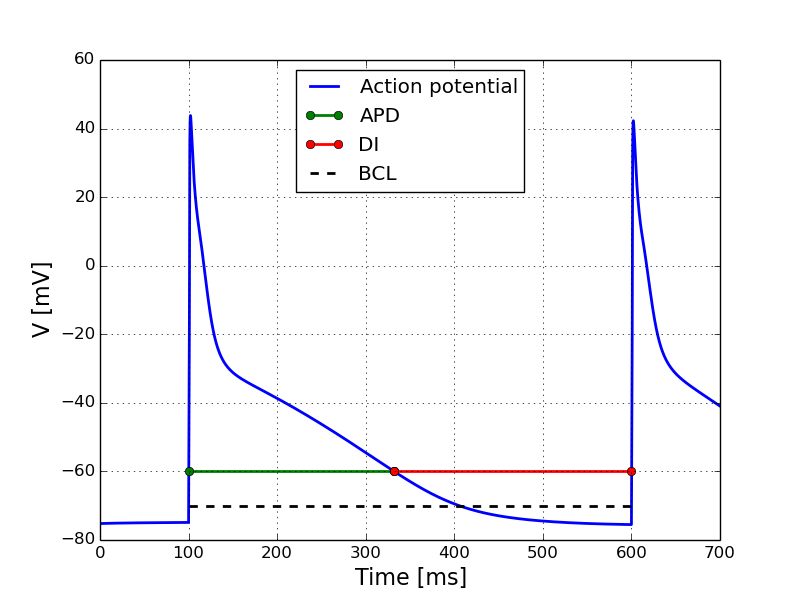
\includegraphics[width=0.7\textwidth]{action_potential}
\caption{Illustration of the APD. The BCL is the duration between every action potential. We divide the BCL into the APD and the diastolic interval.}
\end{figure}

There are different ways of measuring APD$_{90}$ as a function of BCL, that is, different ways to pace the cell model. In S1-S2 pacing, we pace the cell at a given cycle length (S1) for a long time, until the cell is at a steady cycle, when then give a premature stimulus at a shorter cycle length (S2). The APD is measured from the response to the premature stimulus. In contrast we have dynamic pacing, where the cell model is simply paced until steady cycle is reached, the APD is then measured at steady cycle. 

Note that these two pacing protocols will give very different resitution curves for the APD/BCL relationships, due to the interval-duration relationship (see Katz).

\subsubsection*{Code specifics}

To calculate an APD$_90$ restitution curve, we have to scripts, \verb+/0D/pacing_dynamic.py/+ and \verb+/0D/pacing_S1S2.py/+. I think you should focus on the dynamic pacing, as it is quicker. And do both if you get the time. 

You can run the program by changing only the bottom few lines of the script, they should something like this
\begin{lstlisting}
### Example of use 
ode = 'hAM_KSMT_nSR'
#ode = 'hAM_KSMT_cAF'
#ode = 'FK_nSR'
#ode = 'FK_cAF'

BCL_range = range(1000, 295, -5)
dt = 0.01

pacing_dynamic(ode, BCL_range, dt, plot=False)
\end{lstlisting}

First you select which ode cellmodel to use, comment out the three you are not using (comment out by starting the line with the number symbol, \verb+#+). Then you specify what BCL's to compute the APD$_{90}$ for. Now it goes from 1000 to 300 in steps of 5, which is reasonable. Finally we call the script itself, the results will be written to the terminal. The plot keyword can be switched to True if you want to vizualize the results. Note that this makes everything run slower, and the figure must be closed before it moves on to new BCLs. Plotting should just be used to look at the concepts and debugging.

Warning: This script does \emph{not} take into considerations alterans, if the BCL becomes to small, the printed APD$_{90}$ will only be half of the truth. The Koivumäki model produces alterans below a BCL of 300. Below this BCL you should look at the \verb+/0D/alterans.py+-script.

\section*{Effective refractatory period---ERP}

The ERP says something about how long a cell is refractatory, meaning it cannot be stimulated to fire. If we try to stimulate cell model to quickle after an action potential is fired, it will fail to fire. 

In the benchmarking paper (Wilhelms et al, 2013), the ERP is measured in a 1D tissue strand. If you imagine a strand that is stimulated at the left end, a pulse will travel down the strand. If we try to stimulate the left hand side prematurely, no such pulse will travel through the tissue, as the cells are refractatory. The ERP is defined as the smallest time we can wait before a new stimulus will produces a traveling pulse.

In our case, we will define the ERP slightly simpler. As 1D tissue simulations are computationally costly, we would rather just use a 0D cell model. We therefore measure the ERP as the smallest time we can wait between stimulating a single cell model and still get an AP.

The ERP will be a function of the BCL. A cell that is paced slowly, will have a longer refractatory period as a result of a longer APD. To measure the ERP we simply load in the cell model a steady cycle and attempt with a short S2 time. We increase the S2 time step by step untill we can get the cell to fire, this is the ERP for that BCL steady cycle. We then go to the next BCL.

\subsubsection*{Code specifics}

The script is \verb+/0D/effective_refractatory_period.py+. Again, the bottom of the program is what you need to change, it looks something like this

\begin{lstlisting}
BCL_range(300, 1000, 5)

effective_refractatory_period('hAM_KSMT_nSR', BCL_range, erpstart=250)
#effective_refractatory_period('hAM_KSMT_cAF', BCL_range, erpstart=250)
#effective_refractatory_period('FK_nSR', BCL_range, erpstart=50)
#effective_refractatory_period('FK_cAF', BCL_range, erpstart=50)
\end{lstlisting}

From the four last line, select which version you want to run by commentating in and out. The \verb+erpstart+ just designates how low the script should start appyling the S2 stimulus, it cannot be to small, but it can be to big.

\section*{The Conduction Velocity---$C_V$}

The conduction velocity is the speed a signal propagtes through the tissue. Recall that the signal propagation through the tissue is goverened by the monodomain equations, which is an example of a \emph{reaction-diffusion} equation. The system is a set of grid-points, or nodes. Each node describe a collection of cells. As a cell fires an action potential, the rising membrane potential can diffuse to nearby cells, causing them to fire, and this propagates the potential.

The conduction velocity results from a complex set of factors, and is strongly dependant on both the cell model, as well as the tissue properties, such as the diffusion coefficient. There is therefore no simple way of calculating the conduction velocity, and we should simply simulate a propagating wave and measure it from the simulation.

To do this, we denote some sort of threshold for activation, when the potential in a grid point rises above the treshold, we say the cell activates. We then monitor two grid pints, $x_0$ and $x_1$ and measure the time they activate. The conduction velocity is then estimated from
$$C_V \simeq \frac{x_1 - x_0}{t_1 - t_0}.$$

\subsubsection*{Code specifics}

As mentioned, the conduction velocity depends on a lot of different parameters. The cell model itself affects things, as does the tissue diffusion coefficient. The diffusion coefficient, $D$, again depends on numerical properties, such as the time constant and spacing $h$. To set $D$, we simply use the fact that the conduction velocity at a BCL of 1 second should be roughly 750 mm/s. I have already done this and set the diffusion coefficient for both the Koivumäki and FK models.


To simulate the tissue strand, we use 40 grid points, letting each be $0.5$ mm apart, this means we simulate a piece of tissue that is 20 mm long. For every time step, we must solve the ODEs for the cell model for every single grid point, so this computation will be a lot more costly than the 0D measurements.

We start of by loading the steady cycle from the 0D cell model into the tissue strand. But we still should send at least a few pulses through the strand, so that the system approaches a steady cycle for the entire strand. In the program, we do 5 pulses at every given BCL, and print the conduction velocities for each pulse. The last result should be used when plotting the results. As the simulations are so costly in comparsion to the 0D measurements, we do them for fewer BCLs, maybe every 50 or so.

I have also implemented so you can plot in real-time, or not. Plotting is a great way to get a feel for what is going on and how things are working, but they slow down everything considerably. I therefore think you should run the scripts a few time in plot-mode to see how it works, and then without plotting to get a speed-up.

I have also implemented a changing time step, it is important to have a small time step when a cell is firing an action potential, as there are very rapidly changing states which we can only catch properily with a small $\Delta t$, but when the pulse has passed through the grid, and all cells are slowly moving back to resting, we can increase the $\Delta t$. You will see this very clearly if you run the program in plot-mode.

\subsubsection*{Running to code}

Open the file \verb!/1D/measure_cv1D.py!. You should only need to change the lines at the bottom to run the program for different cell models and BCL's. These lines looks something like this
\begin{lstlisting}
solver = TissueStrand('hAM_KSMT_nSR', 0.31, ...)
#solver = TissueStrand('hAM_KSMT_cAF', 0.31, ...)
#solver = TissueStrand('FK_nSR', 0.077, ...)
#solver = TissueStrand('FK_cAF', 0.077, ...)

solver.pulse(1000, num_of_pulses=5, liveplot=True)
\end{lstlisting}

Here, the first line selects what cell model we are using, the rest of the parameters are just so the rest of the script works with the given cell model. You should not mess with these parameters, just choose the different cell models by using one of the first 4 lines (comment in and out using the number symbol \verb+#+).

The sixth line here, is where the script is actually promted to produce results. The first number is the BCL in ms, here it is 1000, that means, 1 second, the \verb+num_of_pulses+ are the number of pulses to use and \verb+liveplot+ denotes whether or not to plot in real time while simulating. In this line, you can change all of these paramters.

The BCL should of course be changed, so that we can get a restitution curve. Live plotting should only be used to study the system, setting it to \verb+False+ yields a big speed-up, so that should be used when simulating for many different BCLs. The number of pulses can be reduced to get a faster running time, but you should first study how much the CV changes from pulse to pulse.

To run for many BCLs in a row, you can use the range function and leave the script running for a long while, for example:
\begin{lstlisting}
solver = TissueStrand('hAM_KSMT_nSR', 0.31, ...)

for BCL in range(1000, 300, -50):
  solver.pulse(BCL, num_of_pulses=5, liveplot=False)
\end{lstlisting}

If you want to also set it up so that the script does this for all the ODEs, you can do it like this
\begin{lstlisting}
solver_list = [TissueStrand('hAM_KSMT_nSR', 0.31, ...),
               TissueStrand('hAM_KSMT_cAF', 0.31, ...),
               TissueStrand('FK_nSR', 0.077, ...),
               TissueStrand('FK_cAF', 0.077, ...)]

for solver in solver_list:  
    for BCL in range(1000, 300, -50):
        solver.pulse(BCL, num_of_pulses=5, liveplot=False)
\end{lstlisting}


\section*{Wavelength}

Finally we have the wavelength. The wavelength is defined as the distance an electrical impulse will travel when the tissue is refractatory. In the paper by Wilhelms et. al they simply compute it as the product of the ERP and the conduction velocity. For simplicity we will do the same here, even though we have found a slightly different ERP.
$$\mbox{WL} = \mbox{ERP} \cdot C_V.$$

\section*{Plotting the results}

So now that we know how to get the measurements, let's look at how to plot them. All the scripts will write the results to the terminal. From the terminal you can copy paste the data into a new script. We could change the scripts to automatically write the data to files, but I figured the `printing to terminal' approach is easier to handle/understand.

Name your new plotscript something descriptive, such as \verb+plot_apd.py+ or \verb+plot_erp.py+. Note the \verb+.py+ file-extension. 

\subsubsection*{Moving the data}
Let us take the dynamic pacing script as an example, the output looks as follows
\begin{lstlisting}
BCL: 1000,  APD: 252.39,   DI: 747.61
BCL: 995,  APD: 250.43,   DI: 744.57
BCL: 990,  APD: 248.77,   DI: 741.23
BCL: 985,  APD: 247.35,   DI: 737.65
BCL: 980,  APD: 246.1,   DI: 733.9
BCL: 975,  APD: 245.01,   DI: 729.99
...
\end{lstlisting}

If we want plot the APD vs the BCL, we need to get these numbers into our plotting scripts, and the data should be defined as a list, as follows
\begin{lstlisting}
APD = [252.39, 250.43, 248.77, 247.35, 246.1, 245.01, ...]
\end{lstlisting}
We also need the BCL, but we do not need to copy it, we can simply write
\begin{lstlisting}
BCL = range(1000, 295, -5)
\end{lstlisting}
or similar, to generate the correct BCLs values. Just how you want to get the APD into a list is up to you, you could do it by hand, or write some code to fix it, or use a smart editors edit+replace functions. If all of this is a lot of work, you could also change the \verb+pacing_dynamic.py+-script to only print the APD values.


\subsubsection*{Plotting the data}
When you have defined both the BCL and APD lists, you can plot them against each other. First you need to import plotting functions
\begin{lstlisting}
from matplotlib.pyplot import *

plot(BCL, APD)  # Plots BCL on x-axis, APD on y-axis
show() # Show the plot on the screen
\end{lstlisting}

If you have APD data for all 4 cell models you can plot them all in the same figure as follows
\begin{lstlisting}
plot(BCL, APD_KnSR)
plot(BCL, APD_KcAF)
plot(BCL, APD_FnSR)
plot(BCL, APD_FcAF)

show()
\end{lstlisting}

\subsubsection*{Prettify the plot}

Once the plot is on screen, you can change it through the menus and then save it. A better approach is to enter your plotscript and do it through code. Between the \verb+plot+ and the \verb+show+ commands, you can add labels/grids/titles/legends and so on. I could for example have the following script

\begin{lstlisting}
plot(BCL, APD_KnSR)
plot(BCL, APD_KcAF)
plot(BCL, APD_FnSR)
plot(BCL, APD_FcAF)

title("Restitution curve, APD90", fontsize=20)
axis([250, 1050, 100, 280]) # Axis are given in xmin, xmax, ymin, ymax order
xlabel()
xlabel("BCL [ms]", fontsize=20)
ylabel("APD [ms]", fontsize=20)
legend(['Koivumaki nSR', 'Koivumaki cAF', 'Fenton-Karma nSR', 'Fenton-Karma cAF'], fontsize=20)
grid()
savefig("restcurve_apd90.png")
show()
\end{lstlisting}

Play around with the different functions and see how they affect the final plot. Note also that you can save in different file formats by changing the ending in the \verb+savefig+ command, you can for example plot in png, pdf or svg. 

Let me know if there is any special way you want your plot to look, and we can make it together. You can see here \url{matplotlib.org/gallery} for inspiration.







































\end{document}
